% =====================================================================================
%  DocROI-Former-QDCT: architecture specification, contributions and benchmark report
%  Compile: pdflatex docroi_former_qdct_spec.tex   (twice, for references)
%  Packages used are all in a standard TeX Live / MiKTeX / Overleaf installation.
% =====================================================================================
\documentclass[10pt,a4paper]{article}

\usepackage[margin=2.1cm]{geometry}
\usepackage[T1]{fontenc}
\usepackage{lmodern}
\usepackage{amsmath,amssymb}
\usepackage{booktabs}
\usepackage{tabularx}
\usepackage{array}
\usepackage{xcolor}
\usepackage{graphicx}
\usepackage{enumitem}
\usepackage{caption}
\usepackage{tikz}
\usetikzlibrary{positioning,arrows.meta,fit,calc}
\usepackage[colorlinks=true,linkcolor=blue!50!black,citecolor=blue!50!black,urlcolor=blue!50!black]{hyperref}

\newcommand{\ours}{DocROI-Former-QDCT}
\newcommand{\R}{\mathbb{R}}
\newcommand{\best}[1]{\textbf{#1}}
\setlist{itemsep=2pt,topsep=3pt}

\title{\textbf{\ours}\\[2pt]
\large Architecture Specification, Contributions and Benchmark Results\\
on the DocTamper Benchmark (DTD Protocol)}
\author{Shivendra Pratap Singh}
\date{19 November 2026}

\begin{document}
\maketitle

% -------------------------------------------------------------------------------------
\begin{abstract}
\noindent
We describe \ours, a 43.9M-parameter dual-stream network for pixel-level localisation of
tampered text in document images. It combines an ImageNet-pretrained PVTv2-B2 RGB
encoder with a forensic residual stream (Bayar + SRM). That stream is augmented with a
quantised JPEG-DCT branch, which reads the coefficient lattice of the final JPEG directly
and is conditioned on its quantisation table. The two streams are fused at four scales by
entity-gated cross-attention with QK-normalisation, and decoded by a progressive guided
upsampling head. The novelties are: (N1) label-free, entity-gated forensic fusion;
(N2) quantisation-table-conditioned (FiLM) injection of exact quantised-DCT evidence into
the residual pyramid; (N3) stabilised cross-modal attention, in which a diagnosed
attention-logit growth is removed by QK-normalisation; (N4) a progressive guided
upsampling decoder with native-resolution SRM edge gating; and (N5) an intra-document
font-consistency objective. The model is trained only on the DocTamper training set, with the
degradation family of the official DTD test protocol. On the official protocol
(grayscale, 1--3 JPEG rounds, minimum quality 75, all 50{,}000 test images, fixed
threshold 0.5), it reaches F1 = 78.1 / 81.5 / 72.3 on TestingSet / FCD / SCD. This is
competitive with DTD (79.2 / 81.6 / 75.4) at two-thirds of its parameter count, but below
ADCD-Net on TestingSet and SCD and well below FFDN. We state explicitly which components
are borrowed and which are ours, and we list the limitations of the current evidence,
notably the absence of component ablations.
\end{abstract}

% -------------------------------------------------------------------------------------
\section{Task and setting}
\begin{itemize}
  \item \textbf{Task.} Binary pixel-level localisation of tampered regions in document
        images. The output is a tamper-probability map at input resolution, thresholded
        at 0.5.
  \item \textbf{Training data.} DocTamperV1-TrainingSet only (120{,}000 images). Of these,
        117{,}500 are used for training and 2{,}500 are held out for validation
        (seed-42 permutation). TestingSet, FCD and SCD are never opened during training.
        DTD's official test quality tables are never read during training.
  \item \textbf{Test protocol.} The DTD protocol~\cite{dtd}, as used by
        FFDN~\cite{ffdn} and ADCD-Net~\cite{adcd}. Each test image is converted to
        grayscale and JPEG-compressed 1--3 times, with per-image quality factors taken
        from DTD's public tables (minimum quality 75). Scoring is at native
        $512\times512$ resolution.
\end{itemize}

% -------------------------------------------------------------------------------------
\section{Novelties}\label{sec:novelty}
\ours\ introduces five design elements. Each is listed with the problem it addresses, its
mechanism, and how it relates to the closest prior work. Table~\ref{tab:novsum} summarises
their cost, and Section~\ref{sec:prov} records which of them are already supported by
controlled experiments.

\paragraph{N1 -- Label-free entity-gated forensic fusion.}
\emph{Problem.} Most pixels of a document image are blank paper. There, the forensic
residuals (Bayar, SRM, DCT) are dominated by acquisition noise: scanner noise, paper
texture, folds and glare. This noise has nothing to do with tampering, whereas text
tampering happens on document content.\\
\emph{Mechanism.} An entity router on the stride-4 RGB features classifies tokens as paper,
text, photo, code or seal. It is trained \emph{without entity labels}: a heuristic Otsu
prior biases the text logit, and everything else is learned end to end through the
relevance path. The router's output is used in three places:
\begin{enumerate}[label=(\alph*)]
  \item A continuous relevance map $\rho$ attenuates forensic features on paper. A floor of
        $\alpha=0.15$ preserves context.
  \item A binary entity mask $m$ restricts the keys of the RGB$\rightarrow$forensic
        cross-attention to content tokens, so RGB queries read forensic evidence only from
        document content.
  \item The same mask up-weights entity pixels in the focal loss.
\end{enumerate}
\emph{Relation to prior work.} ADCD-Net~\cite{adcd} also addresses the disparity between
text and background, through content disentanglement. N1 differs in form: it makes the
document-entity structure an explicit routing signal, which gates both the attention keys
and the residual features.
(Sections~\ref{sec:router} and~\ref{sec:xattn}.)

\paragraph{N2 -- Quantisation-table-conditioned DCT injection into the residual pyramid.}
\emph{Problem.} The same quantised coefficient value means different things at different
compression strengths. Moreover, double-compression traces live in the \emph{integer
lattice} of the coefficients, which mixed-precision arithmetic destroys.\\
\emph{Mechanism.} The stream has five parts:
\begin{enumerate}[label=(\alph*)]
  \item It recomputes the codec's quantised coefficients exactly from the final JPEG's own
        luma plane and table, in fp32 even during bf16 training.
  \item The coefficients are embedded one-hot.
  \item The features are conditioned on $\log Q$ by FiLM. The FiLM layer is
        zero-initialised, so the stream starts as the identity.
  \item The result is added to the forensic pyramid at strides 8 and 4, with nearest
        upsampling so that every pixel keeps its own block's evidence. DCT evidence is thus
        fused with the Bayar/SRM residuals \emph{before} cross-attention.
  \item Flips are applied after compression, which keeps the grid and $|L_b|$ invariant.
\end{enumerate}
The whole stream adds 0.52M parameters (1.2\% of the model).\\
\emph{Relation to prior work.} One-hot quantised coefficients, and the use of the
quantisation table, come from CAT-Net~\cite{catnet} and DTD~\cite{dtd}. Ours are the FiLM
form of the conditioning, the injection into the multi-scale residual pyramid, and the
exactness guarantee under mixed precision.
(Section~\ref{sec:qdct}.)

\paragraph{N3 -- Stabilised cross-modal attention.}
\emph{Problem.} In the RGB-query / forensic-key cross-attention, the spatial-reduction
LayerNorm normalises keys only at stages with $r_i>1$. At stages 3--4 ($r_i=1$) the keys are
unnormalised. In our measurements the attention logits there grew to 157 and 97 (against
5 and 23 at stages 1--2), and training diverged in epoch 5.\\
\emph{Mechanism.} We diagnosed the divergence by reconstructing the seeded data order,
replaying the exact failing batches and measuring per-stage logit magnitudes. The fix is
per-head LayerNorm on queries and keys at every stage, i.e.\ QK-normalisation
(512 parameters). With it, all 88{,}125 updates were finite.\\
\emph{Relation to prior work.} QK-normalisation itself is from Dehghani
\emph{et al.}~\cite{qknorm}. Ours are the diagnosis and its application to cross-modal
attention with spatial reduction.
(Section~\ref{sec:xattn}.)

\paragraph{N4 -- Progressive guided upsampling (PGU) decoder with SRM edge gating.}
\emph{Problem.} Tampered regions in documents are often thin, down to single characters
and strokes, and decoding at stride 4 with plain upsampling blurs their boundaries.\\
\emph{Mechanism.} The decoder works in two steps:
\begin{itemize}
  \item \textbf{Stride 4 $\rightarrow$ 2:} an RGB skip from $S_1$, with an auxiliary output
        for deep supervision.
  \item \textbf{Stride 2 $\rightarrow$ 1, at full resolution:} native-resolution SRM residuals
        enter through a learned $\tanh$ gate conditioned on the decoder features. Edge
        evidence is therefore added only where the decoder deems it relevant.
\end{itemize}
\emph{Relation to prior work.} Forensic-residual-guided boundary refinement at full
resolution inside the decoder.
(Section~\ref{sec:pgu}.)

\paragraph{N5 -- Intra-document font-consistency objective.}
\emph{Problem.} Inserted or edited text often differs subtly in typography from the
authentic text of the same document.\\
\emph{Mechanism.} Stride-4 tokens are projected to $\ell_2$-normalised 128-d embeddings.
Restricted to text tokens (via $m$), an InfoNCE objective pulls the authentic tokens of the
same document together, and a push term separates tampered tokens from that cluster. It is
used only during training and costs nothing at inference.
(Section~\ref{sec:loss}.)

\paragraph{Methodological contribution: leak-proof, protocol-aligned training.}
The training degradations come from the same family as the test protocol, with a
compression curriculum ($q_{\min}$ 95$\rightarrow$75) driven by our own random generator:
\begin{itemize}
  \item DTD's test quality tables are never read during training.
  \item The model is selected on a split held out from the training set.
  \item The selected checkpoint is evaluated once, with SHA-256 fingerprints and per-image
        result files.
\end{itemize}

\begin{table}[!htbp]
\centering
\caption{Novelties at a glance: where each one sits and what it costs.}
\label{tab:novsum}
\begin{tabular}{@{}llrl@{}}
\toprule
 & Novelty & Params & Active at inference \\
\midrule
N1 & Entity router, relevance gates, key masking & 0.41M & yes \\
N2 & Q-conditioned quantised-DCT injection        & 0.52M & yes \\
N3 & QK-normalised cross-modal attention          & 512   & yes \\
N4 & PGU decoder with SRM edge gating             & 2.98M & yes (whole mask head) \\
N5 & Intra-document font-consistency objective    & 0.03M & no (training only) \\
\bottomrule
\end{tabular}
\end{table}

% -------------------------------------------------------------------------------------
\section{End-to-end architecture}

\begin{figure}[t]
\centering
\resizebox{\textwidth}{!}{%
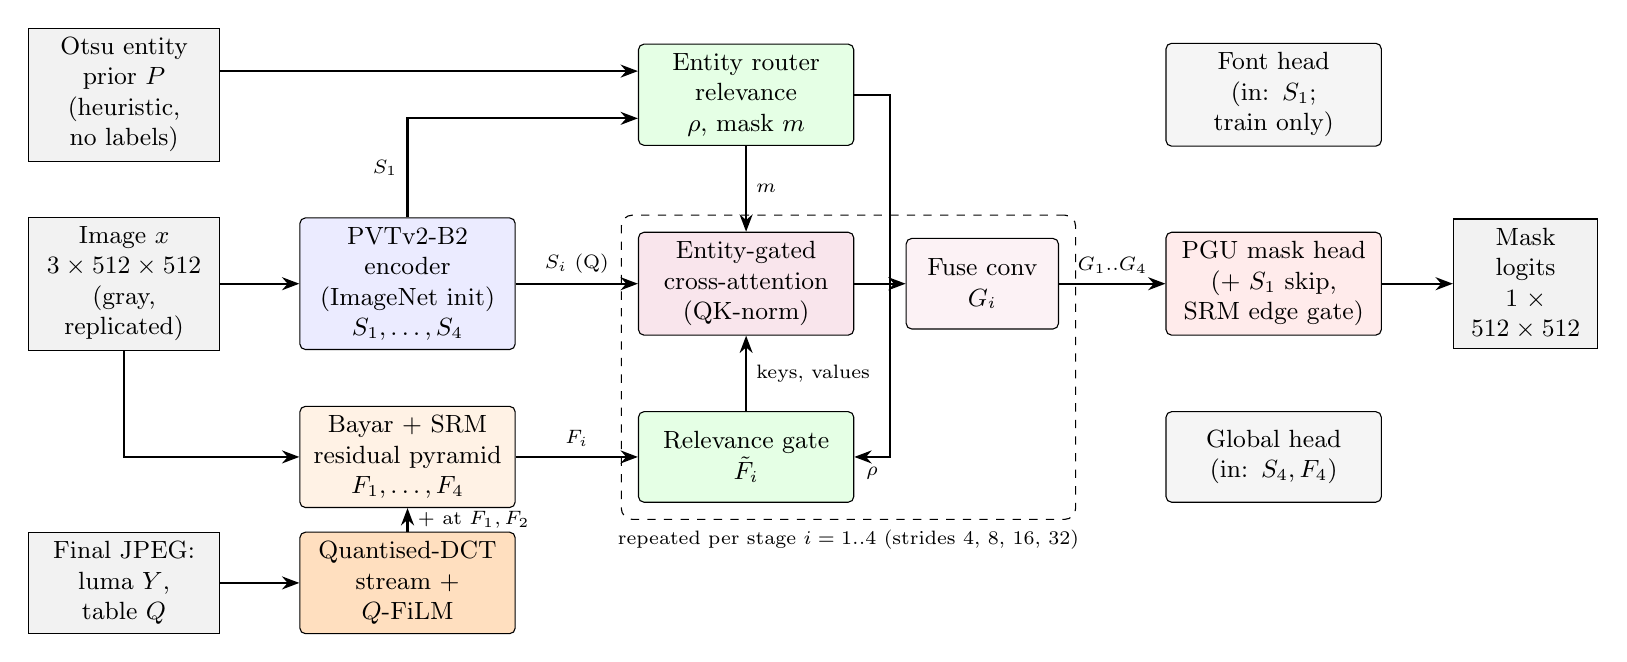
\begin{tikzpicture}[
  font=\small,
  blk/.style={draw, rounded corners=2pt, align=center, minimum height=1.15cm, text width=2.5cm, fill=#1},
  blk/.default={white},
  io/.style={draw, align=center, minimum height=1.0cm, text width=2.2cm, fill=gray!10},
  arr/.style={-{Stealth[length=2.2mm]}, thick},
  lbl/.style={font=\scriptsize, midway}
]
% inputs
\node[io]  (prior) at (0, 4.6)  {Otsu entity prior $P$\\(heuristic, no labels)};
\node[io]  (img)   at (0, 2.2)  {Image $x$\\$3\times512\times512$\\(gray, replicated)};
\node[io]  (jpeg)  at (0,-1.6)  {Final JPEG:\\luma $Y$, table $Q$};
% encoders
\node[blk=blue!8]   (pvt)  at (3.6, 2.2)  {PVTv2-B2 encoder\\(ImageNet init)\\$S_1,\dots,S_4$};
\node[blk=orange!10](res)  at (3.6, 0.0)  {Bayar + SRM\\residual pyramid\\$F_1,\dots,F_4$};
\node[blk=orange!25](qdct) at (3.6,-1.6)  {Quantised-DCT\\stream + $Q$-FiLM};
% router + fusion
\node[blk=green!10] (router) at (7.9, 4.6) {Entity router\\relevance $\rho$, mask $m$};
\node[blk=green!10] (gate)   at (7.9, 0.0) {Relevance gate\\$\tilde F_i$};
\node[blk=purple!10](xattn)  at (7.9, 2.2) {Entity-gated\\cross-attention\\(QK-norm)};
\node[blk=purple!5, text width=1.7cm] (fuse) at (10.9, 2.2) {Fuse conv\\$G_i$};
% heads
\node[blk=red!8]  (mask)   at (14.6, 2.2) {PGU mask head\\(+ $S_1$ skip,\\SRM edge gate)};
\node[blk=gray!8] (glob)   at (14.6, 0.0) {Global head\\(in: $S_4, F_4$)};
\node[blk=gray!8] (font)   at (14.6, 4.6) {Font head\\(in: $S_1$; train only)};
\node[io, text width=1.6cm] (out) at (17.8, 2.2) {Mask logits\\$1\times512\times512$};
% fusion box
\node[draw, dashed, rounded corners=4pt, inner sep=6pt, fit=(gate)(xattn)(fuse)] (box) {};
\node[font=\scriptsize, anchor=north] at (box.south) {repeated per stage $i=1..4$ (strides 4, 8, 16, 32)};
% edges
\draw[arr] (img.east) -- node[lbl, above]{} (pvt.west);
\draw[arr] (img.south) |- (res.west);
\draw[arr] (jpeg.east) -- (qdct.west);
\draw[arr] (qdct.north) -- node[lbl, right]{$+$ at $F_1,F_2$} (res.south);
\draw[arr] ([yshift=3mm]prior.east) -- ([yshift=3mm]router.west);
\draw[arr] (pvt.north) |- node[lbl, pos=0.25, left]{$S_1$} ([yshift=-3mm]router.west);
\draw[arr] (pvt.east) -- node[lbl, above]{$S_i$ (Q)} (xattn.west);
\draw[arr] (res.east) -- node[lbl, above]{$F_i$} (gate.west);
\draw[arr] (gate.north) -- node[lbl, right]{keys, values} (xattn.south);
\draw[arr] (router.south) -- node[lbl, right]{$m$} (xattn.north);
\draw[arr] (router.east) -- ++(0.45,0) |- node[lbl, pos=0.75, below]{$\rho$} (gate.east);
\draw[arr] (xattn.east) -- (fuse.west);
\draw[arr] (fuse.east) -- node[lbl, above]{$G_1..G_4$} (mask.west);
\draw[arr] (mask.east) -- (out.west);
\end{tikzpicture}}
\caption{\ours\ end to end. Only the mask logits are used for localisation and for every
reported metric. The global and font heads are auxiliary training branches (see
Section~\ref{sec:limits}). $S_i$: RGB-stream features; $F_i$: forensic-stream features;
$\rho$: relevance map; $m$: binary entity mask.}
\label{fig:arch}
\end{figure}

Figure~\ref{fig:arch} gives the data flow and Table~\ref{tab:shapes} the tensor shapes at
the training/test resolution ($H=W=512$).

\begin{table}[!htbp]
\centering
\caption{Feature shapes per stage at $512\times512$ input. Cross-attention token counts are
given as queries / keys (after spatial reduction $r_i$).}
\label{tab:shapes}
\begin{tabular}{@{}lccccc@{}}
\toprule
Stage $i$ & Stride & $S_i$ and $F_i$ & SR ratio $r_i$ & Tokens (Q / KV) & Heads $\times$ head dim \\
\midrule
1 & 4  & $64\times128\times128$ & 4 & 16{,}384 / 1{,}024 & $8\times8$  \\
2 & 8  & $128\times64\times64$  & 2 & 4{,}096 / 1{,}024  & $8\times16$ \\
3 & 16 & $320\times32\times32$  & 1 & 1{,}024 / 1{,}024  & $8\times40$ \\
4 & 32 & $512\times16\times16$  & 1 & 256 / 256          & $8\times64$ \\
\bottomrule
\end{tabular}
\end{table}

\subsection{Inputs}
\begin{enumerate}[label=(\alph*)]
  \item \textbf{Image} $x\in\R^{3\times H\times W}$. The protocol makes the document
        grayscale, so the three channels are identical. ImageNet mean/std normalisation is
        applied.
  \item \textbf{Final-JPEG luma and quantisation table} $(Y, Q)$. These are read from the
        last JPEG encoding of the image: the $8\times8$ grid is at $(0,0)$, and $Q$ is in
        natural row-major order. The order Pillow returns the table in is detected at
        runtime against the IJG table.
  \item \textbf{Entity prior} $P\in\{0,1\}^{H\times W}$. This is a heuristic map
        (inverted Otsu threshold, dilation and closing) computed from the input image
        alone. It uses no labels.
\end{enumerate}

\subsection{RGB stream}
A PVTv2-B2 encoder~\cite{pvtv2} (ImageNet-1k initialisation, drop-path 0.1) produces
$S_1,\dots,S_4$ with $(64,128,320,512)$ channels at strides $(4,8,16,32)$.

\subsection{Forensic residual stream}
Two fixed or constrained high-pass front-ends are concatenated into
$R=[\mathrm{Bayar}(x);\,\mathrm{SRM}(x)]\in\R^{6\times H\times W}$:
\begin{itemize}
  \item \textbf{Bayar.} A learnable $5\times5$ constrained convolution~\cite{bayar}, with
        $w_{c}=-1$ and $\sum_{k\neq c} w_k = 1$. As in the original method, the kernel is
        projected back onto the constraint set after every optimiser step. It receives no
        weight decay.
  \item \textbf{SRM.} Three fixed SRM high-pass kernels~\cite{srm}.
\end{itemize}
A convolutional pyramid (two stride-2 Conv--BN--GELU blocks to stride 4, then one
stride-2 block per stage) produces $F_1,\dots,F_4$ with the same shapes as $S_i$.

\subsection{Quantised JPEG-DCT stream \textnormal{(N2)}}\label{sec:qdct}
For every $8\times8$ block $b$ of the final JPEG's luma plane, the stream recomputes the
codec's quantised coefficients. This is done in float32 with mixed precision disabled,
because bf16/fp16 cannot represent the integer lattice exactly:
\begin{align}
C_b(u,v) &= \sum_{x=0}^{7}\sum_{y=0}^{7}\alpha(u)\alpha(v)\,\bigl(Y_b(x,y)-128\bigr)
           \cos\tfrac{(2x+1)u\pi}{16}\cos\tfrac{(2y+1)v\pi}{16},\\
L_b(u,v) &= \min\bigl(\,\bigl|\operatorname{round}\bigl(C_b(u,v)/Q(u,v)\bigr)\bigr|,\;T\bigr),
           \qquad T=20 .
\end{align}
Each $L_b(u,v)$ is one-hot encoded per frequency, giving
$E\in\{0,1\}^{64(T+1)\times\frac H8\times\frac W8}$. This categorical representation was
introduced by CAT-Net~\cite{catnet} and is also used by DTD~\cite{dtd}. The stream then
computes
\begin{align}
Z &= \mathrm{GELU}(\mathrm{BN}(W_e E)) \in \R^{128\times\frac H8\times\frac W8},\\
[\gamma,\beta] &= \mathrm{MLP}\bigl(\log Q/\log 255\bigr),\qquad
Z' = Z\odot(1+\gamma)+\beta \quad\text{(FiLM~\cite{film}, zero-initialised)},\\
D_2 &= \mathrm{Ctx}(Z'),\qquad D_1 = \phi\bigl(\mathrm{Up}^{\mathrm{nearest}}_{\times2}(D_2)\bigr),
\end{align}
where $\mathrm{Ctx}$ is two $3\times3$ Conv--BN--GELU blocks on the block grid and $\phi$ a
$1\times1$ projection to 64 channels. The outputs are injected additively:
$F_1\leftarrow F_1+D_1$, $F_2\leftarrow F_2+D_2$. Horizontal and vertical flips (applied
after compression during training) keep the grid aligned and leave $|L_b|$ unchanged.

\subsection{Entity router and relevance gating \textnormal{(N1)}}\label{sec:router}
A light classifier on $S_1$ predicts five entity logits
$z\in\R^{5\times\frac H4\times\frac W4}$ (paper, text, photo, code, seal). The prior
boosts the text logit: $z_1\leftarrow z_1+2\,P_{\downarrow}$. Two outputs are derived:
\begin{equation}
\rho=\sigma\bigl(g(z)\bigr)\in[0,1]^{\frac H4\times\frac W4},\qquad
m=\mathbb{1}\bigl[\arg\max_c z_c\neq 0\bigr].
\end{equation}
Each forensic feature map is attenuated by relevance and recalibrated channel-wise:
\begin{equation}
\tilde F_i = F_i\odot\bigl(\alpha+(1-\alpha)\,\rho_i\bigr)\odot\sigma\bigl(\mathrm{BN}(W_iF_i)\bigr),\qquad \alpha=0.15 .
\end{equation}
There are no entity labels. The router is trained only through the gradient that reaches
$\rho$; $m$ is an $\arg\max$ and passes no gradient.

\subsection{Entity-gated cross-attention with QK-normalisation \textnormal{(N1, N3)}}\label{sec:xattn}
At each stage, RGB tokens query forensic tokens:
\begin{align}
\hat F_i &= \begin{cases}\mathrm{LN}\bigl(\mathrm{SR}_{r_i}(\tilde F_i)\bigr) & r_i>1\\ \tilde F_i & r_i=1\end{cases},\\
Q &= \mathrm{LN}_q(S_iW_q),\qquad K=\mathrm{LN}_k(\hat F_iW_k),\qquad V=\hat F_iW_v,\\
A &= \operatorname{softmax}\Bigl(\mathcal{M}_{m}\bigl(QK^{\top}/\sqrt{d_h}\bigr)\Bigr),\qquad O_i=(AV)W_o,
\end{align}
where $\mathrm{SR}_{r}$ is a stride-$r$ convolution and $\mathcal{M}_m$ sets the logits of
background keys ($m=0$) to $-10^{4}$. The per-head LayerNorms $\mathrm{LN}_q$ and
$\mathrm{LN}_k$ are QK-normalisation~\cite{qknorm} (512 parameters in total). Stage
features are then fused with the RGB residual:
$G_i=\mathrm{GELU}(\mathrm{BN}(\mathrm{Conv}_{3\times3}[S_i;O_i]))$.

\subsection{Progressive guided upsampling (PGU) mask head \textnormal{(N4)}}\label{sec:pgu}
\begin{enumerate}
  \item \textbf{Stride-4 fusion.} $G_1..G_4$ are projected to 256 channels, upsampled to
        stride 4, concatenated and fused ($3\times3$). A dilated $3\times3$ conv then
        reduces them to 128 channels.
  \item \textbf{Stage A} (stride 4 $\rightarrow$ 2). Bilinear $\times2$, concatenation with a
        projected $S_1$ skip, and a depthwise-separable conv to 96 channels. An auxiliary
        $1\times1$ head here gives deep supervision during training.
  \item \textbf{Stage B} (stride 2 $\rightarrow$ 1). Upsampling to $H\times W$ and a
        depthwise-separable conv to 48 channels $h$. Native-resolution SRM residuals are
        injected through a learned gate, $h\leftarrow h+\tanh(W_g h)\odot\psi(\mathrm{SRM}(x))$.
  \item \textbf{Output.} $3\times3$ conv $\rightarrow$ 24 channels $\rightarrow$ $1\times1$
        conv to the mask logits, with the output bias initialised to $-2.19$ (prior 0.1).
\end{enumerate}

\subsection{Auxiliary heads}
\begin{itemize}
  \item \textbf{Global head.} Average and max pooling of $S_4$ and $F_4$, then an MLP
        ($2048\to512\to256\to1$) giving a document-level logit.
  \item \textbf{Font head.} A two-layer MLP on $S_1$ tokens, producing
        $\ell_2$-normalised 128-d embeddings for an intra-document contrastive loss.
\end{itemize}
Neither head is used at inference or in any reported metric.

\subsection{Parameter budget}
Table~\ref{tab:params} lists the trained parameters per module (43.9M in total).
\begin{table}[!htbp]
\centering
\caption{Trained parameters, counted from the released checkpoint (non-trainable buffers excluded).}
\label{tab:params}
\begin{tabular}{@{}lr@{\qquad}lr@{}}
\toprule
Module & Params (M) & Module & Params (M)\\
\midrule
PVTv2-B2 RGB encoder        & 24.850 & Cross-attention (4 stages) & 1.676\\
Forensic residual pyramid   & 5.370  & Fuse convolutions          & 6.932\\
Quantised-DCT stream        & 0.517  & PGU mask head              & 2.980\\
Entity router               & 0.019  & Global head                & 1.182\\
Relevance gates             & 0.387  & Font head                  & 0.025\\
\midrule
\multicolumn{3}{@{}l}{\textbf{Total}} & \textbf{43.939}\\
\bottomrule
\end{tabular}
\end{table}

% -------------------------------------------------------------------------------------
\section{Training objective}\label{sec:loss}
The total loss is
\begin{equation}
\mathcal{L}=0.30\,\mathcal{L}_{\mathrm{foc}}+0.40\,\mathcal{L}_{\mathrm{dice}}+0.20\,\mathcal{L}_{\mathrm{bnd}}
+0.35\,\mathcal{L}_{\mathrm{aux}}+0.10\,\mathcal{L}_{\mathrm{font}}+0.30\,\mathcal{L}_{\mathrm{glob}} .
\end{equation}
\begin{itemize}
  \item $\mathcal{L}_{\mathrm{foc}}$: focal loss~\cite{focal} with $\gamma=2$ and positive
        weight 1.8. Its pixel weight is $1+0.5\cdot\mathbb{1}[m\lor y]$, i.e.\ up-weighted
        on entity and tampered pixels.
  \item $\mathcal{L}_{\mathrm{dice}}$: soft Dice on images that contain tampering, plus
        $0.5\times$ the mean predicted probability on images that do not.
  \item $\mathcal{L}_{\mathrm{bnd}}$: a boundary-distance penalty
        $\operatorname{mean}\bigl(\varphi_{\mathrm{GT}}\cdot\|\nabla\hat p\|\bigr)$, where
        $\varphi_{\mathrm{GT}}$ is the normalised inside+outside Euclidean distance to the
        ground-truth contour and $\nabla$ is a Sobel operator. It is in the spirit
        of~\cite{boundary}.
  \item $\mathcal{L}_{\mathrm{aux}}$: $0.5\,$focal $+\,0.5\,$Dice on the stride-2 auxiliary
        output.
  \item $\mathcal{L}_{\mathrm{font}}$ (N5): InfoNCE~\cite{infonce} ($\tau=0.07$) that pulls
        authentic text tokens of the same document together, plus a term pushing tampered
        text tokens away from them.
  \item $\mathcal{L}_{\mathrm{glob}}$: BCE on the document label, with positive weight 0.2.
\end{itemize}

% -------------------------------------------------------------------------------------
\section{Training protocol}
\begin{table}[!htbp]
\centering
\caption{Training configuration of the reported checkpoint (run \texttt{qdct\_qkn\_pgu}).}
\label{tab:train}
\begin{tabularx}{\textwidth}{@{}lX@{}}
\toprule
Data & DocTamperV1-TrainingSet: 117{,}500 train / 2{,}500 held-out validation \\
Degradation & Grayscale, then $k\sim\mathcal{U}\{1,2,3\}$ JPEG rounds with
  $q_j\sim\mathcal{U}\{q_{\min},\dots,100\}$ from our own seeded RNG; random horizontal
  and vertical flips ($p=0.5$ each) after compression \\
Curriculum & $q_{\min}$ linear from 95 to 75 over epochs 1--7
  (95, 92, 88, 85, 82, 78), then 75 for epochs 7--12 \\
Resolution & Native $512\times512$, no resizing (required by the JPEG grid) \\
Optimiser & AdamW, weight decay 0.01 (none on norms, biases or Bayar kernels) \\
Learning rate & $6\times10^{-5}$ for both encoders, $3\times10^{-4}$ for router, fusion and
  heads; 1{,}000-update linear warm-up, then cosine decay to 2\% of peak \\
Batch & 4 per step $\times$ 4 accumulation = 16 effective; 12 epochs = 88{,}125 updates
  ($\approx$1.41M samples) \\
Precision & bf16 autocast (the quantised-DCT computation runs in fp32); gradient clipping
  at 1.0; non-finite updates skipped (none occurred) \\
Initialisation & ImageNet-1k PVTv2-B2; all other modules random \\
Model selection & Best held-out validation F1 (DTD formula, threshold 0.5) over 12 epochs;
  selected epoch 11 \\
Hardware & One RTX 5080 (16\,GB); $\approx$80--86 min per epoch; peak memory 9.7\,GiB \\
\bottomrule
\end{tabularx}
\end{table}

\begin{table}[!htbp]
\centering
\caption{Held-out validation (2{,}500 training-set images, own fixed degradation table,
$q_{\min}=75$). The test sets were not used for any choice.}
\label{tab:val}
\begin{tabular}{@{}lcccccccccc@{}}
\toprule
Epoch & 1 & 2 & 3 & 4 & 6 & 8 & 9 & 10 & \textbf{11} & 12 \\
\midrule
Val F1 & 40.1 & 52.5 & 62.9 & 68.7 & 73.3 & 75.5 & 75.8 & 76.6 & \best{76.8} & 76.8 \\
Train $q_{\min}$ & 95 & 92 & 88 & 85 & 78 & 75 & 75 & 75 & 75 & 75 \\
\bottomrule
\end{tabular}
\end{table}

\paragraph{Stability.} An earlier run of the same architecture without QK-normalisation
reached validation F1 of 66.5 at epoch 4, then diverged in epoch 5 (gradient norm
$\sim\!10^{13}$). Inspecting the failing batches showed attention-logit growth in the
cross-attention at stages 3--4 ($r_i=1$), where keys receive no LayerNorm (max $|$logit$|$
157 and 97, against 5 and 23 at stages 1--2). With QK-norm, all 88{,}125 updates were
finite and the gradient norm stayed between about 4.7 and 5.4. The two runs tracked each
other closely before the divergence (epochs 1--2: 40.9 / 53.0 vs.\ 40.1 / 52.5).

% -------------------------------------------------------------------------------------
\section{Evaluation protocol}
The protocol re-implements DTD's evaluation (\texttt{models/eval\_dtd.py}):
\begin{itemize}
  \item Each test image is converted to grayscale and compressed with DTD's public
        per-image qualities, applied oldest first. The tables are
        \texttt{pks/DocTamperV1-}\allowbreak\texttt{<split>\_75.pk}.
  \item The full splits are used: TestingSet 30{,}000, FCD 2{,}000, SCD 18{,}000 images.
  \item Inference is at native resolution, in bf16 (as in training), with a fixed threshold
        of 0.5 and no test-time augmentation.
  \item Metrics:
\end{itemize}
\begin{equation}
P=\frac{1}{N}\sum_{n}\frac{|\hat M_n\cap M_n|}{|\hat M_n|},\qquad
R=\frac{1}{N}\sum_{n}\frac{|\hat M_n\cap M_n|}{|M_n|},\qquad
F=\frac{2PR}{P+R},
\end{equation}
\noindent and IoU is the tampered-class IoU accumulated over all pixels of a split.
The selected checkpoint was evaluated exactly once.

% -------------------------------------------------------------------------------------
\section{Results}

\begin{table}[!htbp]
\centering
\caption{F1 (\%) under the DTD protocol (official per-image qualities, $q_{\min}=75$).
All rows except FFDN and ours are copied from ADCD-Net~\cite{adcd}, Table~1 (values and
parameter counts). FFDN is from~\cite{ffdn}, Table~1 (printed there with two decimals) and
Table~5 (parameters). ``--'': no parameter count published. Mean = plain mean of the three
F1 values, computed by us for every row. $^{\dagger}$Labelled ``CAT-Net'' in ADCD-Net's Table~1; the values are
identical to DTD's Table~4 row ``CAT-Net + CLTD'' (plain CAT-Net there: 70.0 / 55.3 / 63.1).}
\label{tab:main}
\begin{tabular}{@{}lrcccc@{}}
\toprule
Method & Params & TestingSet & FCD & SCD & Mean \\
\midrule
\multicolumn{6}{@{}l}{\emph{Earlier image-forensics methods}}\\
MVSS-Net~\cite{mvss} (ICCV'21)  & 143M & 43.1 & 42.4 & 41.4 & 42.3 \\
CAT-Net + CLTD~\cite{catnet,dtd}$^{\dagger}$ & 114M & 72.1 & 74.1 & 67.0 & 71.1 \\
TruFor~\cite{trufor} (CVPR'23)  & 67M  & 69.1 & 66.7 & 59.4 & 65.1 \\
\multicolumn{6}{@{}l}{\emph{Recent document-tampering methods}}\\
DTD~\cite{dtd} (CVPR'23)        & 66M  & 79.2 & 81.6 & 75.4 & 78.7 \\
PS-Net (via~\cite{adcd})        & --   & 79.8 & 82.7 & 74.1 & 78.9 \\
ADCD-Net~\cite{adcd} (ICCV'25)  & 23M  & 80.6 & 81.5 & 74.0 & 78.7 \\
FFDN~\cite{ffdn} (ECCV'24)      & 140M & \best{86} & \best{92} & \best{81} & \best{86.3} \\
\midrule
\textbf{\ours\ (ours)}          & 43.9M & 78.1 & 81.5 & 72.3 & 77.3 \\
\bottomrule
\end{tabular}
\end{table}

\noindent\textbf{Note on differing published numbers.} Different papers report different
values for the same method. FFDN~\cite{ffdn} re-trained DTD under identical settings
(its Table~1, row DTD$^{*}$) and obtained F1 = 0.79 / 0.85 / 0.75, against the 79.2 / 81.6 /
75.4 listed by ADCD-Net. FFDN also lists CAT-Net at 0.72 / 0.76 / 0.65. We use ADCD-Net's
Table~1 as the single source for all non-FFDN rows, so that those rows come from one table
under one protocol. The ``AVG F1'' column printed in ADCD-Net's Table~1 cannot be reproduced
from its own F1 values for several rows; for example, DTD's F1 values average to 78.7 but
the column prints 77.8. We therefore compute the means ourselves.

\begin{figure}[!htbp]
\centering
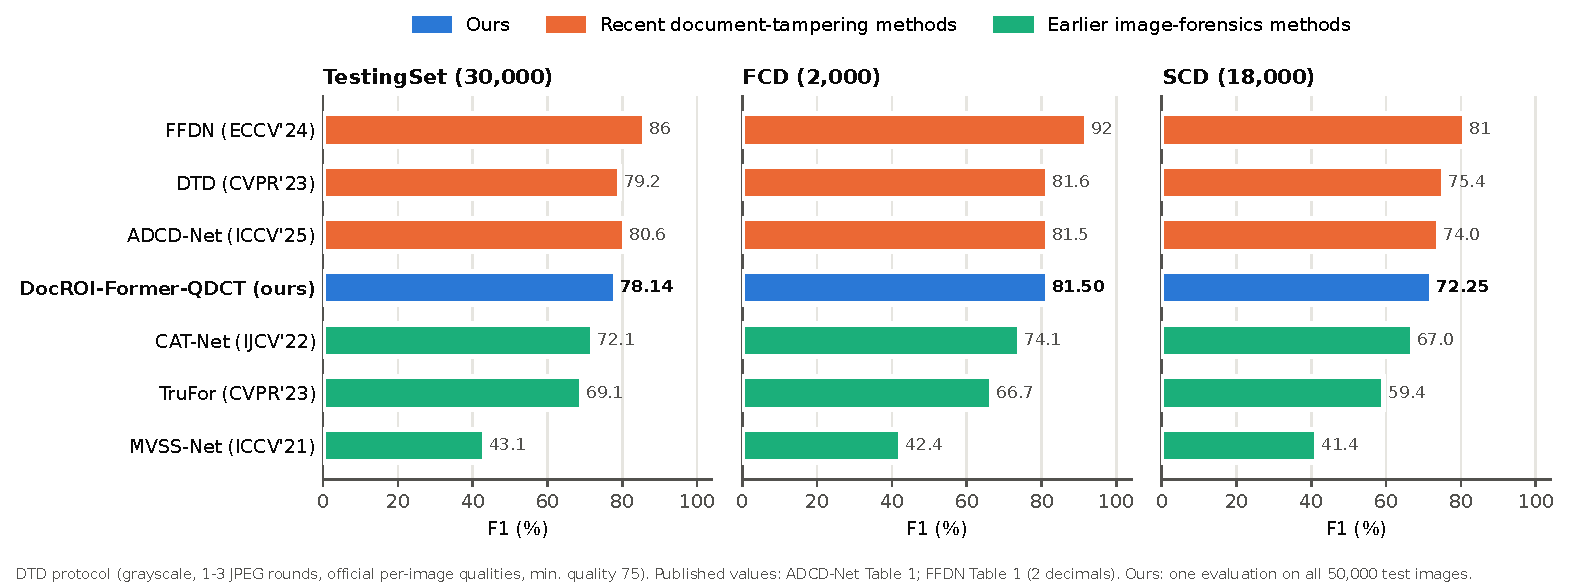
\includegraphics[width=\textwidth]{fig_f1_comparison.pdf}
\caption{F1 per test split under the DTD protocol ($q_{\min}=75$). Sources as in
Table~\ref{tab:main}. Bars start at zero.}
\label{fig:f1}
\end{figure}

\begin{figure}[!htbp]
\centering
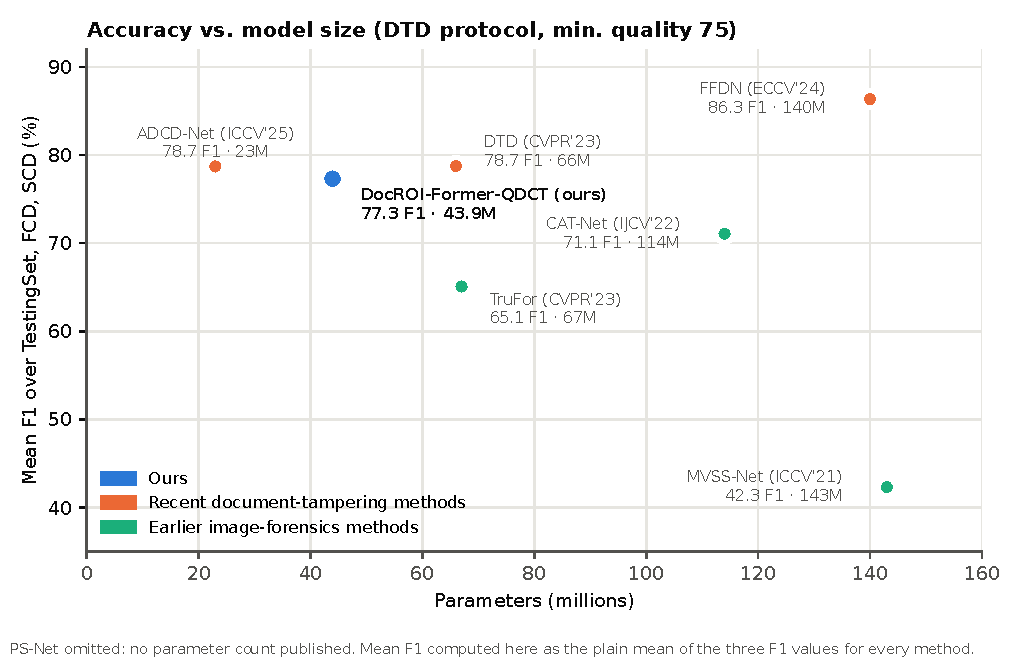
\includegraphics[width=0.78\textwidth]{fig_params_vs_f1.pdf}
\caption{Mean F1 over the three splits against parameter count. PS-Net is omitted because
no parameter count is published. ADCD-Net is both smaller and 1.4 mean F1 more accurate
than ours. DTD is 1.4 mean F1 more accurate with 50\% more parameters. FFDN is the most
accurate, at $3.2\times$ our size.}
\label{fig:params}
\end{figure}

\begin{table}[!htbp]
\centering
\caption{Full metrics of \ours\ (one evaluation run, all test images).}
\label{tab:full}
\begin{tabular}{@{}lrccccc@{}}
\toprule
Split & $N$ & Precision & Recall & F1 & IoU & mIoU \\
\midrule
TestingSet & 30{,}000 & 79.20 & 77.10 & 78.14 & 77.31 & 88.49 \\
FCD        &  2{,}000 & 81.45 & 81.55 & 81.50 & 59.04 & 78.49 \\
SCD        & 18{,}000 & 69.97 & 74.68 & 72.25 & 60.32 & 79.94 \\
\bottomrule
\end{tabular}
\end{table}

\paragraph{Reading of the results.}
\begin{itemize}
  \item The model clearly outperforms the earlier image-forensics methods: CAT-Net + CLTD by 5--7 F1
        on every split, and TruFor and MVSS-Net by more.
  \item It ties ADCD-Net on FCD (81.5) and is 0.1 below DTD there.
  \item It is 1.1 / 3.2 F1 below DTD and 2.5 / 1.7 below ADCD-Net on TestingSet / SCD.
  \item FFDN ($3.2\times$ our size, ConvNeXtV2-B backbone) remains 7.9 / 10.5 / 8.8 F1 ahead.
\end{itemize}
Validation F1 (76.8) and TestingSet F1 (78.1) are consistent, which indicates no selection
leakage.

\paragraph{Previous in-house model.} Our earlier model of the same family
(\texttt{pguoctv3}) was trained at $384\times384$ in colour, with a floating-point DCT
branch and no compression-aware training. Under the same protocol it scored
56.9 / 52.9 / 50.0. It differs in several factors at once, so this gap is not an ablation of
any single component.

\begin{table}[!htbp]
\centering
\caption{Error analysis from per-image results. F1 (DTD formula) by tampered-area fraction
and by number of JPEG rounds. Share = fraction of the split's images.}
\label{tab:breakdown}
\begin{tabular}{@{}lcccc|ccc@{}}
\toprule
 & \multicolumn{4}{c|}{Tampered area / image} & \multicolumn{3}{c}{JPEG rounds} \\
Split & $<$1\% & 1--5\% & 5--15\% & share $<$1\% & 1 & 2 & 3 \\
\midrule
TestingSet & 70.4 & 90.1 & 96.3 & 62\% & 80.6 & 78.4 & 75.3 \\
FCD        & 68.1 & 83.6 & 81.8 & 11\% & 82.9 & 81.5 & 80.1 \\
SCD        & 69.0 & 79.0 & 83.1 & 70\% & 73.9 & 71.9 & 71.0 \\
\bottomrule
\end{tabular}
\end{table}

\paragraph{Where the gap comes from.} Localisation of regions above 1\% of the image is
strong (90--96 F1 on TestingSet). Almost all of the deficit relative to DTD and ADCD-Net
comes from very small edits, under 1\% of the image area (for example a single character).
These make up 62\% of TestingSet and 70\% of SCD; 10.3\% of TestingSet images contain no
correctly detected tampered pixel. Robustness to compression is good: from one to three
JPEG rounds, F1 drops by 5.3 on TestingSet, 2.8 on FCD and 2.9 on SCD.

% -------------------------------------------------------------------------------------
\section{Evidence status of each novelty}\label{sec:prov}
Table~\ref{tab:novelty} separates what is taken from prior work from what is specific to
this model (N1--N5, Section~\ref{sec:novelty}). The ``Evidence'' column states what
currently supports each claim.

\begin{table}[!htbp]
\centering
\caption{Components, origin, and current evidence.}
\label{tab:novelty}
\small
\begin{tabularx}{\textwidth}{@{}>{\raggedright\arraybackslash}p{3.3cm}>{\raggedright\arraybackslash}p{3.0cm}>{\raggedright\arraybackslash}X>{\raggedright\arraybackslash}p{2.7cm}@{}}
\toprule
Component & Prior art & Specific to this work & Evidence \\
\midrule
PVTv2 RGB encoder & \cite{pvtv2} & -- (standard backbone) & -- \\
Bayar + SRM residuals & \cite{bayar,srm} & Constraint projection after every step (fixed an
  earlier NaN divergence) & Training stability \\
Quantised-DCT one-hot coefficients, Q-table use & \cite{catnet,dtd} & \textbf{N2}: FiLM
  conditioning on $\log Q$ (zero-init); injection into the residual pyramid at strides 8
  and 4; exact lattice under mixed precision & System result only \\
Entity router + relevance gating & content disentanglement~\cite{adcd} (different form) &
  \textbf{N1}: label-free document-entity routing (heuristic prior + learned classifier)
  that attenuates forensic features on paper & System result only \\
Entity-gated cross-attention & SR-attention~\cite{pvtv2} & \textbf{N1}: RGB$\rightarrow$forensic
  cross-attention whose keys are masked to document entities & System result only \\
QK-normalisation & \cite{qknorm} & \textbf{N3}: diagnosis of logit growth at $r_i=1$ stages
  without key LayerNorm; fix applied to cross-modal attention & Divergence removed
  (measured) \\
PGU mask head with SRM edge gate & -- & \textbf{N4}: two-step guided upsampling with
  native-resolution SRM edge injection and deep supervision & System result only \\
Font contrastive loss & InfoNCE~\cite{infonce} & \textbf{N5}: intra-document
  authentic-vs-tampered token objective & System result only \\
Protocol-aligned training & \cite{dtd} (protocol) & Quality curriculum
  $q_{\min}$ 95$\rightarrow$75 with our own RNG; test tables never read & System result only \\
\bottomrule
\end{tabularx}
\end{table}

\noindent\textbf{Summary of claims we can make today.}
\begin{enumerate}
  \item A 43.9M-parameter model that matches DTD on FCD and comes within 1--3 F1 of
        DTD/ADCD-Net on TestingSet/SCD, with two-thirds of DTD's parameters.
  \item Five novelties (N1--N5, Section~\ref{sec:novelty}), whose combination produces the
        result above. Their individual contributions are \emph{not yet} isolated by
        ablation.
  \item An identified and fixed training instability in cross-modal attention: QK-norm at
        the stages without key normalisation.
\end{enumerate}

% -------------------------------------------------------------------------------------
\section{Limitations and open items}\label{sec:limits}
\begin{enumerate}
  \item \textbf{No component ablations.} Every row marked ``system result only'' in
        Table~\ref{tab:novelty} still needs a controlled ablation, i.e.\ the same recipe
        with that component removed, before it can be claimed as a contribution in a
        publication.
  \item \textbf{Single run, single seed.} There are no error bars. The compared methods
        also report single runs.
  \item \textbf{Re-implemented protocol.} The evaluation follows DTD's script step by step
        but was not validated by reproducing a published number with DTD's released
        weights.
  \item \textbf{Small edits.} F1 is about 70 on regions under 1\% of the image, which
        accounts for most of the gap to the state of the art.
  \item \textbf{Auxiliary heads.} Almost every DocTamper training image contains tampering,
        so the global (document-level) head is effectively untrained for authentic
        documents and must not be used as a classifier. The font head serves only as a
        training regulariser.
  \item \textbf{Domain.} DocTamper is predominantly Chinese-language documents. Behaviour on
        other document types, such as identity documents, and the false-alarm rate on
        authentic documents have not been measured for this checkpoint.
\end{enumerate}

% -------------------------------------------------------------------------------------
\section*{Appendix: reproducibility record}
\begin{itemize}
  \item \textbf{Checkpoint:} \texttt{runs/qdct\_qkn\_pgu/best\_docroi\_former\_qdct\_qdct\_qkn\_pgu.pth}
        (epoch 11).\\ SHA-256: {\footnotesize\texttt{76810b6110bf1d42e93247f0f592c346}\allowbreak\texttt{b4740be183f6861561f8e2edba5f0563}}
  \item \textbf{Quality tables (SHA-256):}
  \begin{itemize}
    \item TestingSet: {\footnotesize\texttt{b34d4b52bb5f10eced18d832144eecdb}\allowbreak\texttt{18972d48fd692a8547ca8162ff55a751}}
    \item FCD: {\footnotesize\texttt{db67bd20045099927df492918ed3e340}\allowbreak\texttt{ab55c5a4f0d043f459e39aa6e1b73b0d}}
    \item SCD: {\footnotesize\texttt{3ddad77ca6757427aca10ae69e8e0bf7}\allowbreak\texttt{92917c332f23e5aef143fdbfde7bddf7}}
  \end{itemize}
  \item \textbf{Evaluation record:} run \texttt{20261119\_113438\_dtd\_q75}, folder\\
        \texttt{reports/dtd\_protocol/FINAL\_RESULT\_ALLTHREELOGGED\_RESULT/}. It holds
        \texttt{eval.log}, \texttt{summary.csv}, \texttt{summary.json}, and one
        per-image CSV per split (50{,}000 rows in total).
  \item \textbf{Training and evaluation commands:}
{\footnotesize
\begin{verbatim}
python train_academic.py --run_name qdct_qkn_pgu --init imagenet --resolution 512 \
    --epochs 12 --batch_size 4 --grad_accum 4 --dct quantized --qk_norm 1 --seed 0
python evaluate_dtd_protocol.py --checkpoint <ckpt> --infer_size 0 \
    --datasets TestingSet,FCD,SCD --minq 75 --threshold 0.5
\end{verbatim}
}
  \item \textbf{Software and hardware:} PyTorch 2.12 (dev build, CUDA 12.8), single NVIDIA
        RTX 5080.
\end{itemize}

% -------------------------------------------------------------------------------------
\begin{thebibliography}{99}\small
\bibitem{dtd} C.~Qu \emph{et al.}, ``Towards robust tampered text detection in document
  image: New dataset and new solution,'' in \emph{CVPR}, 2023.
\bibitem{ffdn} Z.~Chen \emph{et al.}, ``Enhancing tampered text detection through frequency
  feature fusion and decomposition,'' in \emph{ECCV}, 2024.
\bibitem{adcd} K.~Wong \emph{et al.}, ``ADCD-Net: Robust document image forgery localization
  via adaptive DCT feature and hierarchical content disentanglement,'' in \emph{ICCV}, 2025.
\bibitem{catnet} M.-J.~Kwon \emph{et al.}, ``Learning JPEG compression artifacts for image
  manipulation detection and localization,'' \emph{IJCV}, 2022.
\bibitem{mvss} X.~Chen \emph{et al.}, ``Image manipulation detection by multi-view
  multi-scale supervision,'' in \emph{ICCV}, 2021.
\bibitem{trufor} F.~Guillaro \emph{et al.}, ``TruFor: Leveraging all-round clues for
  trustworthy image forgery detection and localization,'' in \emph{CVPR}, 2023.
\bibitem{pvtv2} W.~Wang \emph{et al.}, ``PVT v2: Improved baselines with pyramid vision
  transformer,'' \emph{Computational Visual Media}, 2022.
\bibitem{bayar} B.~Bayar and M.~C.~Stamm, ``Constrained convolutional neural networks: A new
  approach towards general purpose image manipulation detection,'' \emph{IEEE TIFS}, 2018.
\bibitem{srm} J.~Fridrich and J.~Kodovsk\'y, ``Rich models for steganalysis of digital
  images,'' \emph{IEEE TIFS}, 2012.
\bibitem{qknorm} M.~Dehghani \emph{et al.}, ``Scaling vision transformers to 22 billion
  parameters,'' in \emph{ICML}, 2023.
\bibitem{film} E.~Perez \emph{et al.}, ``FiLM: Visual reasoning with a general conditioning
  layer,'' in \emph{AAAI}, 2018.
\bibitem{focal} T.-Y.~Lin \emph{et al.}, ``Focal loss for dense object detection,'' in
  \emph{ICCV}, 2017.
\bibitem{boundary} H.~Kervadec \emph{et al.}, ``Boundary loss for highly unbalanced
  segmentation,'' in \emph{MIDL}, 2019.
\bibitem{infonce} A.~van den Oord, Y.~Li and O.~Vinyals, ``Representation learning with
  contrastive predictive coding,'' arXiv:1807.03748, 2018.
\end{thebibliography}

\end{document}
